\providecommand{\paper}[1]{#1}
\providecommand{\thesis}[1]{}

\paper{
\newcommand{\pth}{.}
\newcommand{\this}{paper}
\documentclass[oribibl]{lncs/llncs}
\usepackage{amssymb, graphicx, float, textcomp}
\include{\pth/local}
\title{\Huge Visualising DNA with Rauzy Projections}
%\author{H. J. Hoogeboom, W. A. Kosters, J. F. J. Laros\\
%        and S. M. Verduyn Lunel
%        \vspace{10pt}\\
%        Leiden Institute of Advanced Computer Science (LIACS)\\
%        Universiteit Leiden, The Netherlands\\
%        \texttt{jlaros@liacs.nl}}
\author{J.F.J. Laros\inst{1} \and H.J. Hoogeboom\inst{1} \and W.A. Kosters\inst{1} \and S.M. Verduyn Lunel\inst{2}}
\institute{Leiden Institute of Advanced Computer Science (LIACS), Universiteit Leiden \and Mathematical Institute, Universiteit Leiden \\
\email{jlaros@liacs.nl}}
%\address{Leiden Institute of Advanced Computer Science\\
%         Universiteit Leiden, The Netherlands}
%\email{jlaros@liacs.nl}
\date{\today}
\frenchspacing
%\setlength{\parindent}{0pt}

%\newtheorem{theorem}{Theorem}
%\newtheorem{lemma}[theorem]{Lemma}
%\newtheorem{corollary}[theorem]{Corollary}
%
%\theoremstyle{definition}
%\newtheorem{example}[theorem]{Example}
%\newtheorem{definition}[]{Definition}
%\newtheorem{remark}[theorem]{Remark}
%\newtheorem{conjecture}[theorem]{Conjecture}

\begin{document}

\maketitle
}

\paper{
\begin{abstract} \noindent
}
We propose a novel visualisation method for DNA and other long sequences over a
small alphabet, which is based on the construction of the family of Rauzy
fractals for infinite words. We use this technique to find repeating structures
of widely varying length in the input string as well as the identification of
coding segments. Other properties of the input can also come to light using
this technique.
\paper{
\end{abstract}
}

\section{Introduction}\label{dv:sec:introduction}
Projections of high dimensional structures onto a low dimensional surfaces
(e.g. 2D, 3D) are commonly used to make structures in the data insightful. 

Recognising patterns in long sequences is difficult for humans. The longer the
sequence, the harder it gets. Furthermore, if the alphabet used for this
sequence is small, the task gets even harder. If there are (small) deviations
allowed in the patterns to be recognised, it will be nearly impossible without
the aid of some sort. 

In this \this, we introduce a visualisation technique for DNA sequences using a
projection onto a surface to investigate patterns in the DNA.

In Section~\ref{dv:sec:background} we explain the underlying idea of making
fractals out of infinite words, which we adapt for our purposes in
Sections~\ref{dv:sec:dna}\paper{ and~\ref{dv:sec:ell}}. In Section~\ref{dv:sec:ex} we
show the visualisation results. Finally, related work is discussed in
Section~\ref{dv:sec:rel} and we conclude in Section~\ref{dv:sec:concl}.

\section{Background}\label{dv:sec:background}
In this section, we describe the approach of Rauzy~\cite{Rau} to construct a
fractal from an infinite word.

Given a finite alphabet $\Sigma$, we denote the set of all finite
strings over this alphabet as $\Sigma^*$. In this section we take 
$\Sigma = \{0, 1, 2\}$.

Rauzy investigated the so-called tribonacci substitution:

\begin{eqnarray*}
\sigma: \left\{ \begin{array}{lll}
0 &\rightarrow& 01\\
1 &\rightarrow& 02\\
2 &\rightarrow& 0
\end{array} \right.
\end{eqnarray*}
This substitution induces a \emph{homomorphism}, again denoted by $\sigma$,
from $\Sigma^*$ to $\Sigma^*$. It is uniquely extended to $\Sigma^*$ by
requiring $\sigma(u \cdot v) = \sigma(u) \cdot \sigma(v)$ for all $u, v \in
\Sigma^*$, where $\cdot$ denotes concatenation of strings.

Since $0$ is a prefix of $\sigma(0)$, the following holds: $\sigma^n(0)$ is a
prefix of $\sigma^{n + 1}(0) (n = 1, 2, \ldots)$. Also $|\sigma^n(0)| \ge n
\rightarrow \infty$ when $n \rightarrow \infty$. Therefore $(\sigma^n(0))_{n
\in \mathbb{N}}$ defines a unique infinite word that has $\sigma^n(0)$ as
finite prefix for each $n \in \mathbb{N}$. This word is invariant under the
substitution (where we simultaneously substitute each letter). We call this
word an accumulation point or fixed point of this substitution. For the given
substitution $\sigma$, we get the word $010201001020101020100\ldots$ as fixed
point.

Rauzy used this infinite word to make a plot in
3-dimensional space, starting in $(0, 0, 0)$ and doing one step in the
$x$-direction whenever a $0$ occurs, a step in the $y$-direction when a $1$
occurs and a step in the $z$-direction when a $2$ occurs. All steps are of
equal length. This results in a so-called \emph{broken halfline} which
``approximates'' a halfline $\ell$ starting in the origin. The existence of
this halfline is discussed in~\cite{Rau}.

Now we can take the plane through the origin which is perpendicular to the line
$\ell$ and project the broken halfline onto this plane. This results in the
\emph{Rauzy fractal}, depicted in Figure~\ref{dv:fig:rauzy}. The colour
of the projected points depends on whether the next step from the original
point on the broken halfline is in the $x$-, $y$-, or $z$-direction. 

\begin{figure}
\hspace{.25cm}
\begin{minipage}[t]{.45\textwidth}
\begin{center}
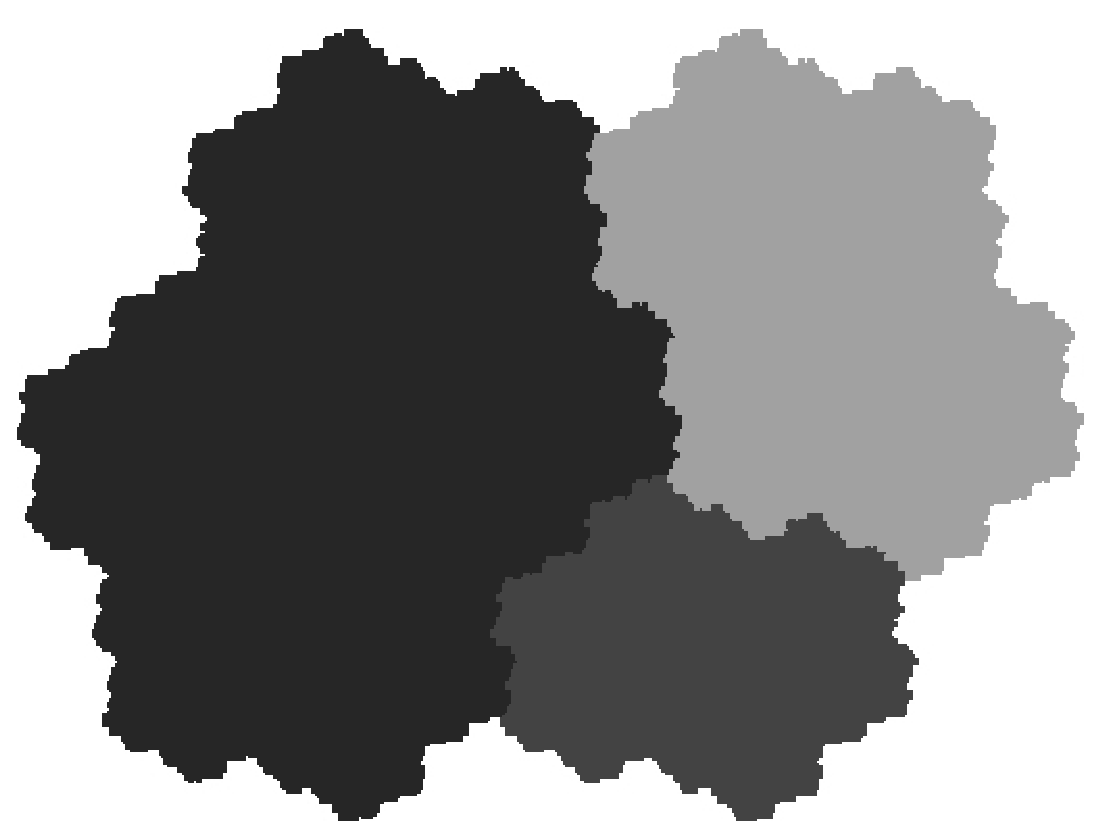
\includegraphics[width=\textwidth]{\pth/017_g}
\end{center}
\caption{Standard Rauzy fractal} \label{dv:fig:rauzy}
\end{minipage}
\hfill
\begin{minipage}[t]{.45\textwidth}
\begin{center}
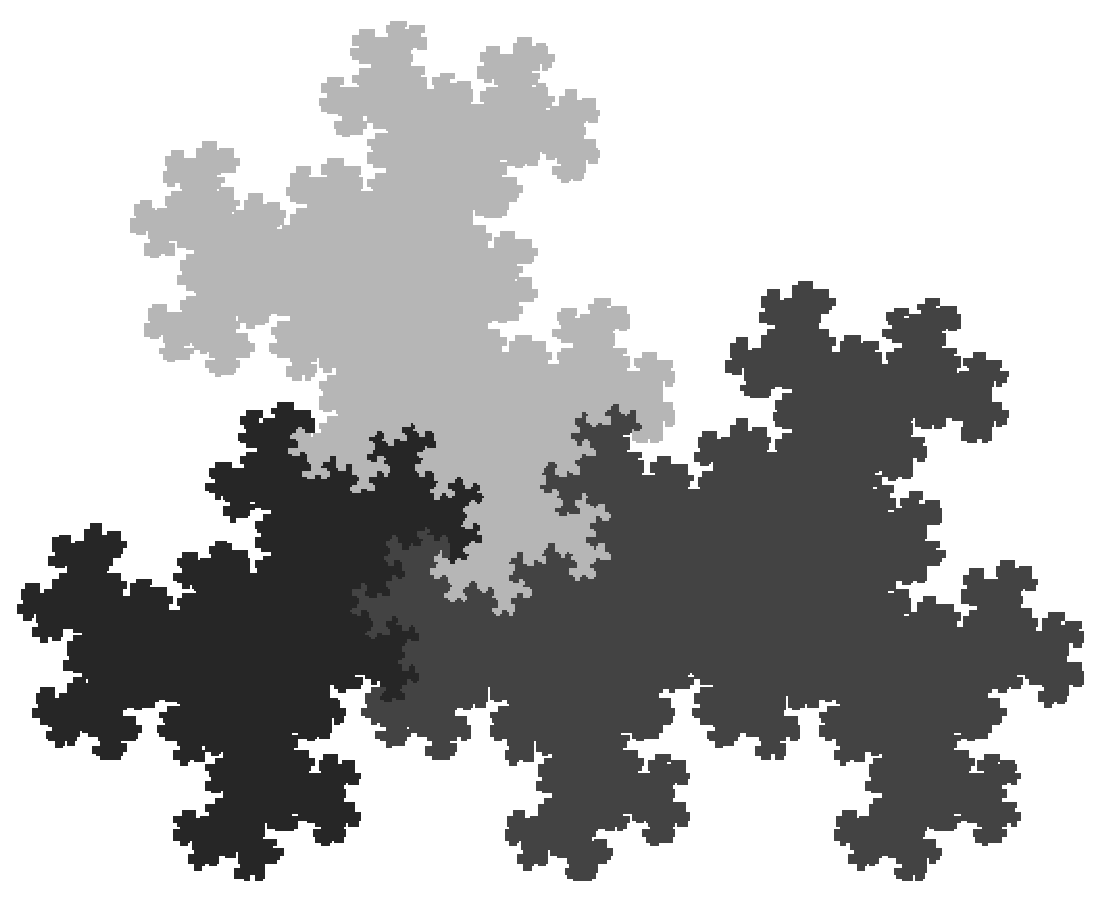
\includegraphics[width=\textwidth]{\pth/006_g}
\end{center}
\caption{A ``Rauzy'' fractal using a different substitution} 
\label{dv:fig:rauzy2}
\end{minipage}
\hspace{.25cm}
\end{figure}

When a different substitution is used, fractals can be made in the same
manner. We see such a fractal in Figure~\ref{dv:fig:rauzy2}. The substitution
in applied here is:

\begin{eqnarray*}
\sigma: \left\{ \begin{array}{lll}
0 &\rightarrow& 01\\
1 &\rightarrow& 2\\
2 &\rightarrow& 0
\end{array} \right.
\end{eqnarray*}

\section{Application to DNA}\label{dv:sec:dna}
We can apply a similar technique to a DNA sequence. First we have to
make a plot in 4-dimensional space by associating each nucleotide (\texttt{A},
\texttt{C}, \texttt{G} and \texttt{T}) with one of the spacial dimensions and
analogous to the construction described above we have to build a broken
halfline, but now in four dimensions.

Then we can make a 2- or 3-dimensional projection by either choosing a plane or
a hyperplane through the origin and by projecting the broken halfline upon that
(hyper)plane.

One big difference with the Rauzy approach in three dimensions is that the
choice of the line $\ell$ which approximates the broken halfline is not
pre-determined. A DNA string does not have the nice mathematical properties
that the tribonacci fixed point possesses, so there is no clear preference for
$\ell$. One choice could be the line going through the begin- and endpoint of
the broken halfline. This is possible since a DNA string is finite. However,
this will result in different choices for $\ell$ for different DNA strings.
This might not be the best choice. Therefore, we shall look (only) at a
solution that uses a fixed $\ell$ for every input.

\paper{
\section{The choice of the line $\ell$}\label{dv:sec:ell}
As mentioned in the previous section, we have multiple possibilities to choose
a line $\ell$ along which we project our data.
}
If $\ell$ is chosen well, we expect to find the following in the projected
image:
\begin{itemize}
\item A non-predictable walk for information rich parts of the DNA.
\item A true random walk for random parts.
\item Lines (or approximate lines) for repeating parts of the DNA.
\item Large copies of substrings in the DNA, that can be easily visualised.
\end{itemize}

\noindent
The term \emph{non-predictable walk} should be taken loosely, because we know
that coding DNA (and therefore information rich DNA) has a higher
\texttt{GC}-content than other parts of the DNA. Therefore, the walk will tend
to go into the \texttt{GC}-direction, and second, DNA is clearly not random.

Since we have so much freedom in the choice of $\ell$, we can also look at the
projection in the following way: In principle, we can choose four vectors in 
the plane and use these four vectors to make the projection. Associate the 
first vector with the nucleotide \texttt{A}, the second one with \texttt{C},
and so on. Now, to make an insightful projection, we want the four vectors to
have the following properties:
\begin{itemize}
\item The vectors should be of comparable length.
\item The four vectors should add up to $0$.
\item Every subset of three vectors should be independent.
\end{itemize}

\noindent
By adhering to these properties, we arrive in the same point if we
consecutively plot a combination of all four letters, this would thus indicate
a perfect repeat of those four letters, or a repeat of all four letters in any
order.

When using an interactive program like \texttt{gnuplot} to visualise the data,
the angle between the vectors can easily be adjusted (especially when making
2-D projections) by stretching the image. We must, however, make sure that the
vectors are not chosen parallel to the axes, otherwise the stretching will only
result in the alteration of the length of the vectors. This property of
interactive programs, along with the ability to zoom in, makes the exploration
of dense areas in our visualisation possible.

We made an interactive web application available via~\cite{DNAV}. This
demonstration has access to the first $1,\!000,\!000$ base pairs of the Human
chromosome~1 and can visualise any substring. For performance reasons, we added
a \emph{step size} to make the rendering of large substrings possible. The data
is located on the webserver and it is kept small for practical purposes. Making
more data available will have no effect on the visualisation application (e.g.,
this will not make the application slower).

\section{A number of DNA sequence visualisations}\label{dv:sec:ex}
In this section, we shall make several projections, on both 2- and
3-dimensional hyperplanes. In each case, we choose a set of vectors for the
nucleotides \texttt{A}, \texttt{C}, \texttt{G} and \texttt{T}. We denote these
vectors by $v_\mathtt{A}$, $v_\mathtt{C}$, $v_\mathtt{G}$ and $v_\mathtt{T}$
respectively.

\subsection{Projections in three dimensions}
For three dimensions, there is, apart from symmetry, a natural choice of the
projection line $\ell$ and therefore the resulting vectors. This set is the one
that defines a tetrahedron (centred at the origin), as shown in
Table~\ref{dv:tab:th}. In other words, the convex hull of the set of endpoints
of these vectors forms a tetrahedron. All vectors in this set have the same
length, the four of them sum up to $0$ and each three-element subset is
independent. Furthermore, the vectors are uniformly distributed, i.e., the
angle between each pair of vectors is equal.

\begin{table}[H]
\begin{displaymath}
\left(
\begin{array}{rrrr}
1 & -1 & -1 &  1\\
1 & -1 &  1 & -1\\
1 &  1 & -1 & -1\\
\end{array}
\right)
\end{displaymath}
\caption{Vertices of a tetrahedron}
\label{dv:tab:th}
\end{table}

We associate the first column with $v_\mathtt{A}$, the second column with 
$v_\mathtt{C}$ and so on. In the remainder of this section, we shall use these
vectors for our projections.

As input for our three dimensional projection, we use the first $160,\!000$
nucleotides of the human Y-chromosome~\cite{GN} (build 18). This results in the
picture shown in Figure~\ref{dv:fig:y-3d}. For clarity, we include the four
vectors and the associated nucleotides in the visualisation. 

\thesis{
\begin{figure}
\vspace*{-15mm}
\hspace{.25cm}
\begin{minipage}[t]{.45\textwidth}
%\begin{center}
\hspace{-1cm}
\includegraphics[angle=270, width=1.3\textwidth]{\pth/y-3d.ps}
\caption{The first $160,\!000$ nucleotides of the human Y-chromosome}
\label{dv:fig:y-3d}
%\end{center}
\end{minipage}
\hfill
\begin{minipage}[t]{.45\textwidth}
%\begin{center}
\hspace{-1cm}
\includegraphics[angle=270, width=1.3\textwidth]{\pth/y2-3d.ps}
\caption{The first $160,\!000$ nucleotides of the human Y-chromosome; viewing angle differs from that in Figure \ref{dv:fig:y-3d}}
\label{dv:fig:y2-3d}
%\end{center}
\end{minipage}
\hspace{.25cm}
\end{figure}
}
\paper{
\begin{figure}[H]
\vspace*{-15mm}
\begin{center}
\includegraphics[angle=270, width=\textwidth]{\pth/y-3d.ps}
\caption{The first $160,\!000$ nucleotides of the human Y-chromosome}
\label{dv:fig:y-3d}
\end{center}
\end{figure}

\begin{figure}[H]
\vspace*{-15mm}
\begin{center}
\includegraphics[angle=270, width=\textwidth]{\pth/y2-3d.ps}
\caption{The first $160,\!000$ nucleotides of the human Y-chromosome; viewing andle differs from that in Figure \ref{dv:fig:y-3d}}
\label{dv:fig:y2-3d}
\end{center}
\end{figure}
}

In Figure~\ref{dv:fig:y2-3d}, we see the exact same data and projection, but
shown from a different angle. This figure is a better representation of the
data, more structures can be seen directly from this angle. We shall discuss
the findings in detail in Section~\ref{dv:subsec:ex2d}.

\begin{figure}[H]
%\vspace{-1cm}
\vspace*{-15mm}
\begin{center}
\includegraphics[angle=270, width=.85\textwidth]{\pth/1-3d.ps}
\caption{Offset $40,\!000$--$100,\!000$ of the human chromosome 1}
\label{dv:fig:1-3d}
\end{center}
%\end{minipage}
%\hspace{.25cm}
\end{figure}

In Figure~\ref{dv:fig:1-3d}, we see a part of the first human chromosome.
Again, we shall discuss the findings in detail in Section~\ref{dv:subsec:ex2d}.

\subsection{Projections in two dimensions}\label{dv:subsec:ex2d}
Since, in two dimensions, there is no way to choose four vectors of equal
length, of which all subsets are independent, we must choose the vectors in
such a way that the lengths differ, to satisfy the independency constraint.
Therefore we can choose, e.g., the following vectors for \texttt{A}, \texttt{C},
\texttt{G} and \texttt{T} respectively: $(5, 7)$, $(-7, 6)$, $(8, -4)$ and
$(-6,-9)$. By choosing these vectors, we have the property that every pair is
independent, and the lengths are comparable. For practical purposes, we have
chosen integer coordinates.

As input we again use the first $160,\!000$ nucleotides of the human
Y-chromosome~\cite{GN} (build 18). This results in the following projection:

\begin{figure}[H]
\begin{center}
\includegraphics[angle=270, width=.85\textwidth]{\pth/160000}
\caption{The first $160,\!000$ nucleotides of the human Y-chromosome}
\label{dv:fig:160000}
\end{center}
\vspace*{-5mm}
\end{figure}

The numbers in this plot denote the offset in the DNA, the plot starts in $(0,
0)$. We immediately see that two of the three hypotheses from
Section~\paper{\ref{dv:sec:ell}}\thesis{\ref{dv:sec:dna}} can be verified for
this input data. There are lines, which denote (approximate) repeats. For
example, the line that starts somewhere near $(-3000, 4500)$ and ends in
$(-7500, 9000)$ contains a large number of approximate copies of the string
\texttt{CCCCGCTCCTCCCCTCGGGACCACCCCAGA}. In the region near $(23000, 9000)$,
marked by the offset $115000$, we see a part where the walk seems random.
Moreover, we can see an extremely large substring from $(-2500, 3000)$ to
$(5500, 8500)$ (approximately offset $5000$ to $25000$) that repeats itself
from $(11000, 6000)$ to $(18500, 11500)$ (approximately offset $93000$ to
$107000$).

\begin{figure}[H]
%\vspace{-1mm}
\begin{center}
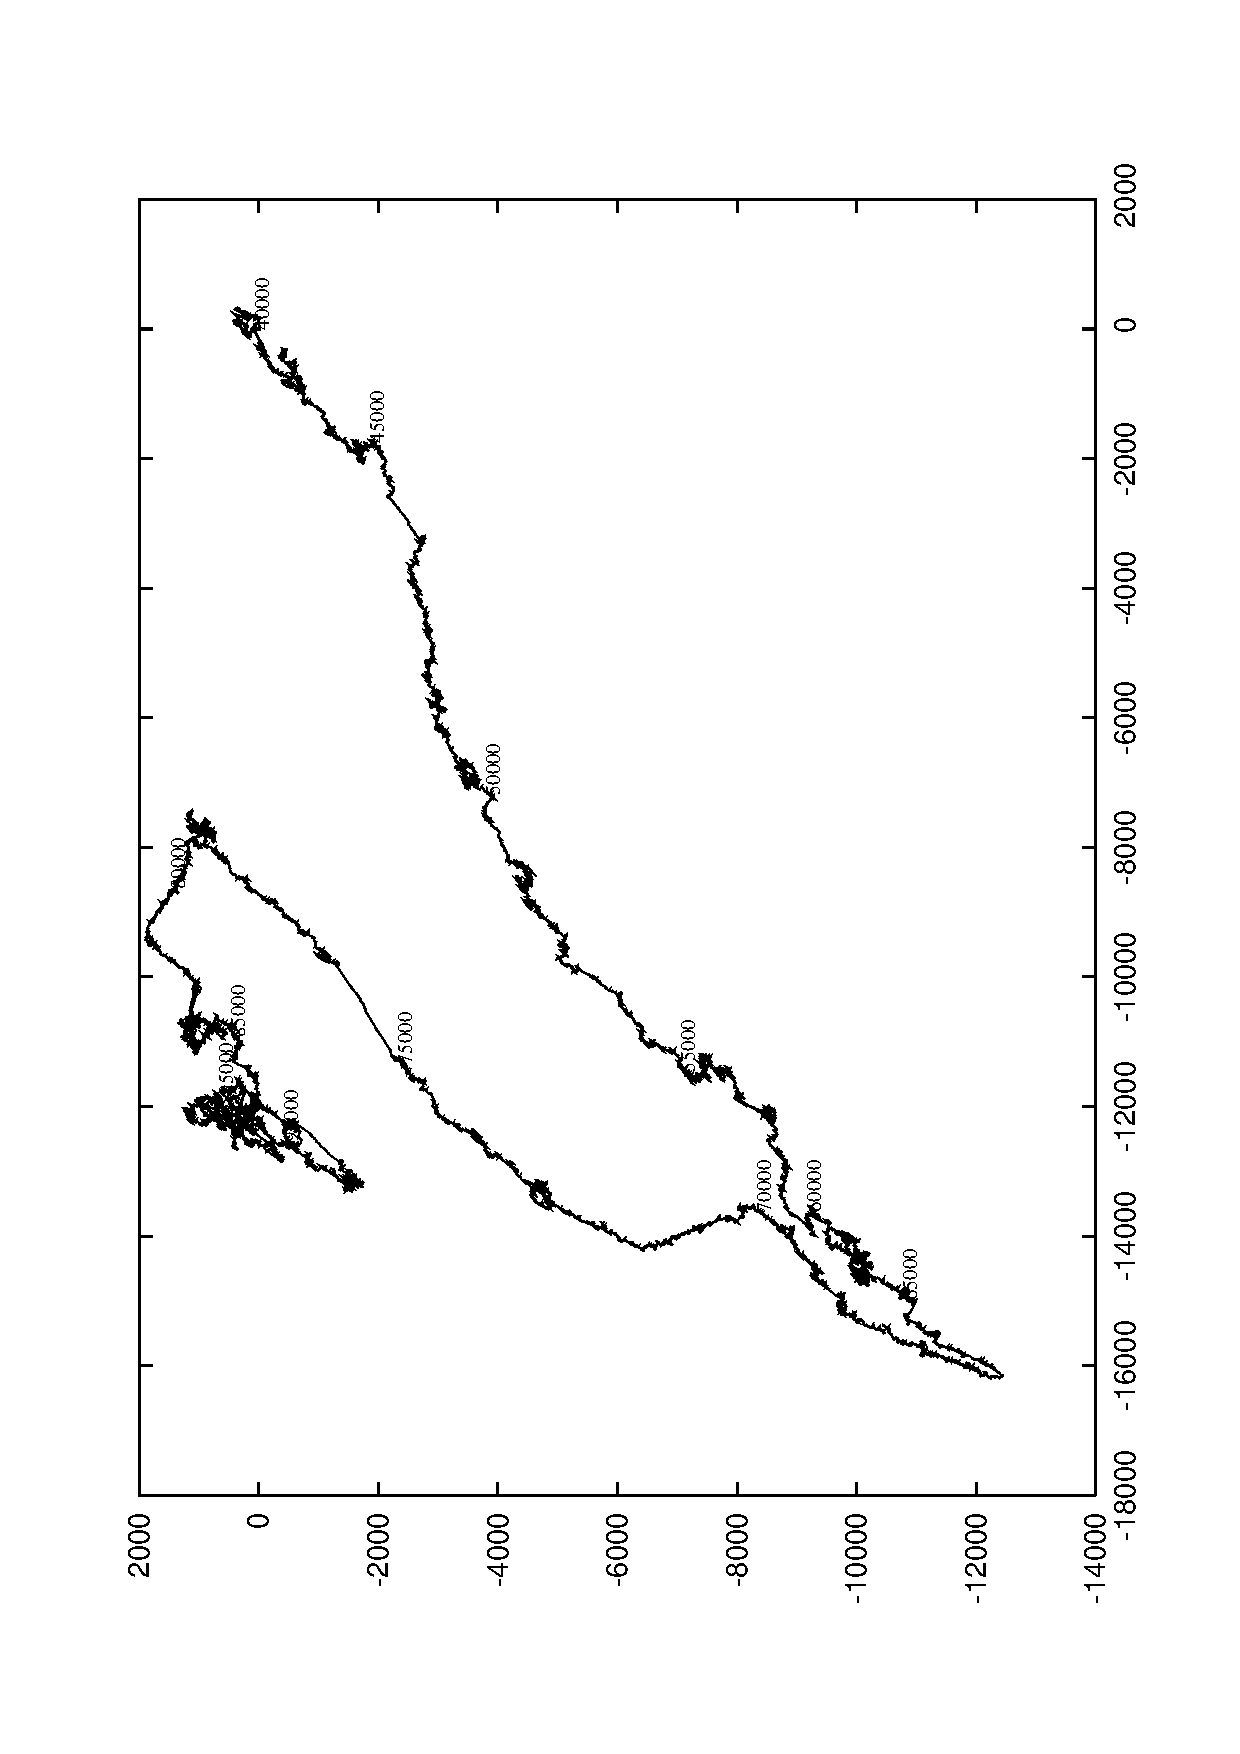
\includegraphics[angle=270, width=.85\textwidth]{\pth/chr1}
\caption{Offset $40,\!000$--$100,\!000$ of the human chromosome 1}
\label{dv:fig:chr1}
\end{center}
\vspace*{-5mm}
\end{figure}

In Figure~\ref{dv:fig:chr1} we see a part of the human chromosome~1. No large
repeats are noticeable in this part of the genome, but we can clearly see some
short repeating sequences. These sequences appear to be lines in our
visualisation. The string \texttt{TTC} for example, is repeated a number of
times from position $(-2600, -2200)$ to $(-3200, -2700)$. Another obvious short
repeat, \texttt{AAG}, can be seen from position $(-11200, -2200)$ to $(-9700,
-1200)$, approximately.

\begin{figure}[H]
%\vspace{-1mm}
\begin{center}
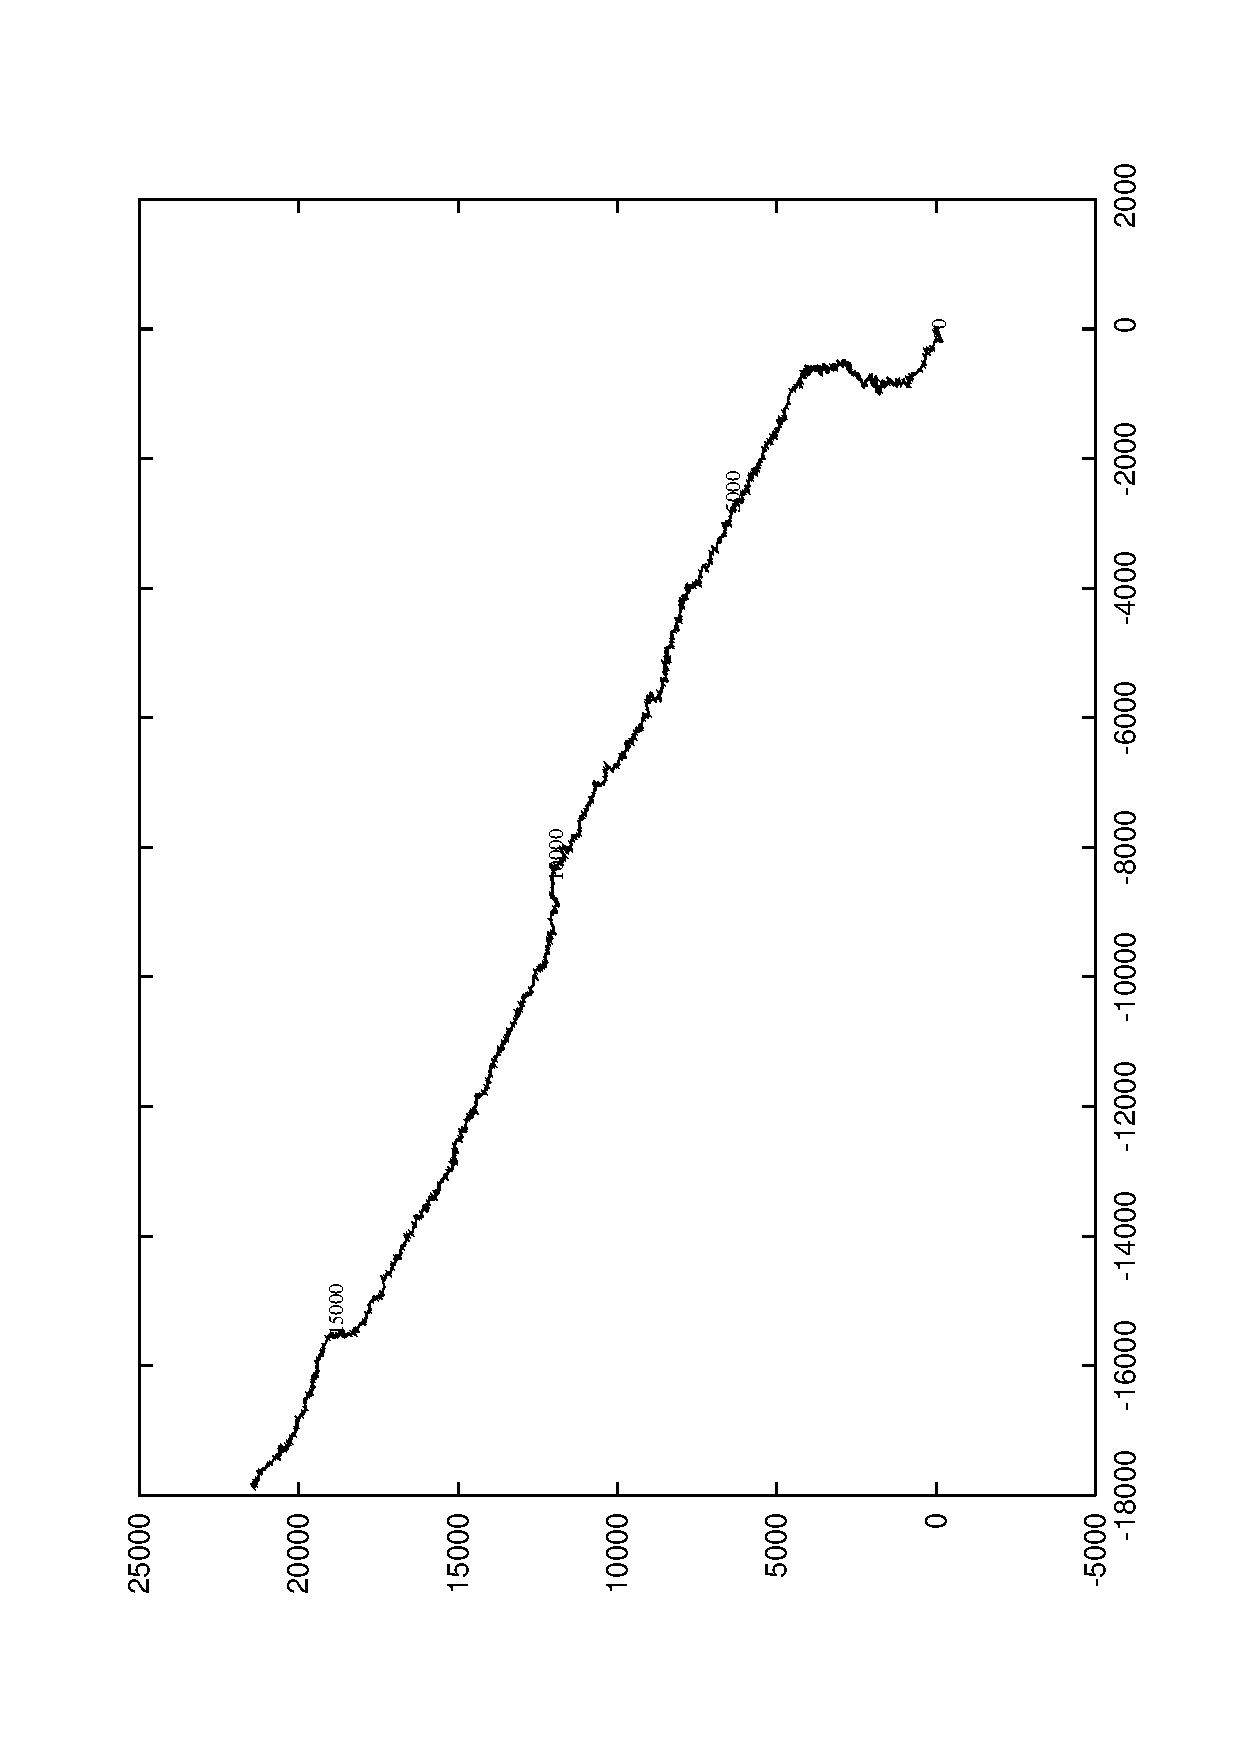
\includegraphics[angle=270, width=.85\textwidth]{\pth/chrM}
\caption{The complete mitochondrial DNA}
\label{dv:fig:chrM}
\end{center}
\vspace*{-5mm}
\end{figure}

In Figure~\ref{dv:fig:chrM}, we see the DNA of mitochondria found in the human
species. The most noticeable is the drift in the \texttt{C}-direction. Further
analysis shows that this is due to the relatively low content of
\texttt{G}-nucleotides in the mitochondrial DNA ($13\%$ versus $25$--$31\%$ for
the other nucleotides).

\section{Related work}\label{dv:sec:rel}
In the DNA-rainbow~\cite{BK} project, plots of DNA were made by assigning a
colour to a nucleotide; green for Adenine, red for Thymine, white for Guanine
and blue for Cytosine. Undetermined positions were given a grey colour. Then
the nucleotides were plotted to a standard bitmap with a width of $770$ pixels.
The resulting pictures, viewable with any picture viewer and/or editor, give a
colourful impression of the DNA. Most of the pictures appear random, but in
some parts, repeating parts of the genome can be seen in the form of diagonal
lines. A nice property of this approach is that \texttt{GC}-rich areas (which
are associated with encoding DNA), can be spotted right away. 

An obvious shortcoming of this approach is the fixed width of the picture.
Short repeating sequences which have a total length of under $770$, will not
stand out. Very long repeating sequences will not stand out either, since it 
will look like a random block that is repeated. 
However, for the detection of short repeating sequences (that are repeated for
a large number of times), this approach seems very well suited.

In~\cite{IVD}, several visualisation methods are investigated. One of them is
essentially the same as in the previously described project, but here the width
of the columns can be changed to detect (small) repeats of different length.
Other visualisation methods include information hiding by using less colours,
and usage of expert knowledge to emphasise some subsequences, like start and
stop codons. Furthermore, a translation to amino acids can also be made with
this technique. According to the authors of~\cite{IVD}, their proposed method
is useful for sequences up to a length of $2,\!000$ base pairs.

In~\cite{MS}, several visualisation techniques are reviewed: the ``random
walk'' visualisation, as well as a fractal visualisation and a visualisation
based on entropy-like parameters which are calculated within a sliding window.
The ``random walk'' resembles the visualisation discussed in this \this, with
the exception that the directions that are associated with the nucleotides are 
fixed and the technique is limited to two dimensions.

\section{Conclusions and further research}\label{dv:sec:concl}
In this paper we have proposed a visualisation for long strings of DNA. The
technique indeed has the properties we expected. We have shown that all our
hypotheses were confirmed; the simple repeats indeed show up as lines in our
visualisation. What we did not expect were the large repeats (the thick lines
mentioned in Section~\ref{dv:sec:ex}), although it is a rather nice result.
Furthermore, we detected a large approximate repeat on the first part of the
Y-chromosome. This repeat is already known by genetic experts, but it is nice
to have detected it with no excessive calculation, like the alignment of two
large sequences, providing hope for further exploration of DNA in this way.

As recommendations for further research, we suggest using colours as an extra
coding scheme. By doing this, we can see the direction of a line in our 
visualisation. For example, it is hard to distinguish between simple repeats
\texttt{AAG} and \texttt{CTT} because they are almost each others inverse. The
lines resulting from these repeats will have approximately the same slope
(see Figure~\ref{dv:fig:chr1} for an example of this), although their content
is different. The only ways to distinguish them at this point is to measure the
exact slope, or by looking at the offsets and thereby finding the orientation
of the line. By using a colour coding scheme, the colour of the line will
represent the orientation directly.

%An other interesting extension would be to project the DNA onto a 3-D surface,
%instead of a 2-D one. A 3-D engine would be required to explore the 
%visualisation, but since we lose less information, the produced images will be
%more insightful.
An other interesting extension would be to make the line $\ell$ along which we
project the 4-D structure onto a surface a parameter that can be changed in
real time. A potential user could try to find a projection, better suited for
his or her purposes.

\paper{
\subsection*{Acknowledgements}
This research is part of the DALE (Data Assistance for Law Enforcement) 
project as financed in the ToKeN program from the Netherlands Organization 
for Scientific Research (NWO) under grant number 634.000.430.\\

\bibliography{../../bibliography}{}
\bibliographystyle{plain}

\end{document}
}
